\documentclass[11pt,a4paper]{article}

\usepackage[utf8]{inputenc}
\usepackage[T1]{fontenc}
\usepackage{lmodern}
\usepackage{amsmath,amssymb,amsfonts,amsthm,bm}
\usepackage{graphicx}
\usepackage{booktabs}
\usepackage{hyperref}
\hypersetup{hidelinks}
\usepackage{url}
\usepackage[margin=1in]{geometry}
\usepackage{enumitem}
\setlength{\emergencystretch}{2em}

\title{Structure-Aware Neural Decoding for the X-Cube Fracton Code\\
\large Finite-Size Results for Logical-Parity Inference}

\author{Brian Guarraci\\
  Galatheus\\
  \texttt{brian@galatheus.com}}

\date{October 2026 revision}

\begin{document}
\maketitle

\begin{abstract}
We study learned logical recovery for the X-cube fracton code under
code-capacity $X$ noise with perfect syndrome measurements. A weight-shared
3D convolutional network reads the cube ($Z$) syndrome and uses a
line-aggregation head (\textsc{AxisLineonHead}) to predict the $6L-3$
logical-$Z$ parities in a fixed axis-aligned basis. Models are trained
separately at each code size and physical error rate. Across
$L\in\{3,4,6,8,10\}$ and $p\in\{0.03,0.05\}$, three-seed evaluations
on disjoint test splits give lower block failure and mean per-sector
logical error than the all-zero baseline, BP+OSD-0, and our simplified
Brown--Williamson-inspired implementation (BW-naive).
At $p=0.03$, mean per-sector error decreases monotonically from $0.042$
to $0.003$ over the tested sizes. Block failure increases from $0.306$
at $L=3$ to $0.343$ at $L=4$, then decreases to $0.118$ at $L=10$.
At $p=0.05$, block failure instead increases with size, despite the
improvement in per-sector error from $L=4$ onward. A single-seed
$L=3$ ablation finds comparable performance for line-aggregation and
coordinate-convolution heads; global pooling performs like the all-zero
baseline. This supports retaining spatial information but does not isolate
line aggregation as the unique mechanism. The results demonstrate
finite-size learned recovery in the tested regime. They do not establish
a threshold, superiority to a validated implementation of the published
Brown--Williamson decoder, cross-size transfer, or a passive quantum memory.

\end{abstract}

\section{Introduction}
\label{sec:intro}
This work began with a classical communication question: if a receiver
already has a useful model of a source, how much instance-specific evidence
must a sender transmit? A syndrome can identify a set of compatible signals,
while a shared prior ranks or samples plausible reconstructions within that
set. The companion occupancy-grid work investigates this idea using learned
spatial priors, with spectral and coarse side information in the reported
experiments. Its objective is reconstruction quality under a bit budget.

Quantum error correction poses a related inference problem with a different
target. A syndrome constrains the physical errors that may have occurred;
the noise model supplies their prior probabilities. Successful recovery
requires the correct logical class, rather than a plausible replacement
for an unknown quantum state. This distinction is essential: classical
perceptual plausibility is not a quantum recovery criterion.

Here we study that inference task for the X-cube code~\cite{vijay2016}.
Its cube syndrome has a regular three-dimensional representation, while
the logical labels in our chosen basis are associated with wrapping lines.
We test a convolutional decoder that preserves this spatial organization
through a line-aggregation readout. Existing code-specific decoders exploit
the same code's planar constraints through matching~\cite{brown2019}; a
single surface-code-style matching problem over pairs of defects does not
directly represent the four-defect patterns of the channel studied here.
The overlapping weight-12 cube checks also make this a useful setting in
which to compare with a generic BP+OSD-0 baseline.

\paragraph{Contribution and scope.}
We report three-seed finite-size measurements for code-capacity $X$ noise,
using both whole-block failure and mean error over a fixed logical basis.
The learned decoder improves on the implemented baselines at every tested
operating point. Its block failure decreases from $L=4$ to $L=10$ at
$p=0.03$ but increases over that range at $p=0.05$. Models are trained
separately at each $(L,p)$; the results do not measure transfer between
sizes or an asymptotic threshold. The head ablation is evidence about
retaining position information, with stronger mechanism tests left open.

The companion gauge note characterizes the classical axial-parity
codespace, and the surface-code paper studies neural decoding budgets.
These motivate a shared question about useful inductive biases; neither
the classical theorem nor a physical equivalence between these systems
is required for the X-cube benchmark. Passive storage and self-correction
remain separate questions about Hamiltonian dynamics and memory lifetime.

\section{Background: the X-cube code and the decoding task}
\label{sec:background}
The X-cube code~\cite{vijay2016} places its qubits on the $3L^3$ edges of a
periodic $L \times L \times L$ cubic lattice. The stabilizer group is generated
by (i) $X$-type ``cross'' operators --- per vertex, the four-edge planar cross
in each of the $xy$, $yz$, $xz$ planes (two independent per vertex, since the
third is their product), and (ii) $Z$-type ``cube'' operators --- the product of
the twelve edges of each elementary cube. The code is CSS
($H_X H_Z^\top = 0$ over $\mathbb{F}_2$) and we verify
$k = N - \mathrm{rank}(H_X) - \mathrm{rank}(H_Z) = 6L - 3$ for all
simulated sizes $L \in \{2,3,4,5,6,8,10\}$ (giving
$k = 9, 15, 21, 27, 33, 45, 57$), matching the known ground-state
degeneracy on the 3-torus.

We study the code-capacity bit-flip ($X$) channel at rate $p$, detected by
the cube ($Z$) stabilizers. The cube syndrome has exactly $L^3$ bits --- one
per cube center --- so it is naturally an $L \times L \times L$ scalar field,
a direct fit for a 3D convolutional decoder with no temporal axis. The
decoding label is the vector of $6L-3$ logical-$Z$ parities of the error,
$\ell_j = \langle \mathrm{logical}_Z^{(j)}, e \rangle \bmod 2$; the decoder
predicts these per-sector classes from the syndrome field. We report
\emph{block failure} (any sector wrong) and the mean \emph{per-sector
logical error rate} (LER).

\paragraph{Why this is decoding, not classification.} Predicting the $6L-3$
logical-$Z$ parities is the full decoding output, not a proxy. Given a syndrome
$s$, fix once a syndrome-consistent representative (``pure error'') $R(s)$
derived from $H_Z$; the residual $e \oplus R(s)$ then lies in the
logical$+$stabilizer group, so the only remaining freedom is which logical coset
it occupies. In the experiments below the network is trained to predict the raw
logical parities $\langle \mathrm{logical}_Z^{(j)}, e\rangle$ of the sampled
error. Equivalently, an explicit recovery using an arbitrary $R(s)$ applies the
logical correction with parity
$\hat\ell_j \oplus \langle \mathrm{logical}_Z^{(j)}, R(s)\rangle$; if $R(s)$ is
chosen with zero logical-$Z$ parities this offset vanishes. A per-sector logical
error occurs precisely when the predicted parity is wrong. This defines a logical-class decoder. The implemented loss is a sum
of binary cross-entropies, and each output is thresholded separately.
At the population optimum, these outputs estimate the marginal probabilities
$P(\ell_j=1\mid s)$; their separate modes minimize expected per-sector
error. They do not in general maximize the joint probability $P(\ell\mid s)$,
which is the decision rule for minimizing block failure. We therefore
report block failure separately and do not identify this training objective
with exact joint maximum-likelihood coset decoding.

\section{Classical motivation and the algebraic connection}
\label{sec:bridge}
The classical axial-parity result is
$\ker H=\mathrm{image}(\partial_x\partial_y\partial_z)$ over
$\mathbb{F}_2$ on a periodic $n^3$ voxel lattice, with
$\mathrm{rank}(H)=3n^2-3n+1$. Writing
$T=\partial_x\partial_y\partial_z$, a voxel residual can be parameterized
as $T\phi$, with the redundancy $\phi\mapsto\phi+\kappa$ for
$\kappa\in\ker T$. This is an exact statement about the classical
constraint set and its parameterization.

Subsystem constraints and redundant potentials also occur in fracton
models~\cite{vijay2016,pretko2017}. The classical identity alone does not
identify the codec with a particular quantum gauge theory or the X-cube
phase: that would require a mapping of local degrees of freedom, operators,
and physical constraints. No such identification is assumed here.
What carries across the paper family is a statistical question: how should
a decoder combine a prior with syndrome evidence while preserving the
geometry relevant to its target?

\section{Decoder and baselines}
\label{sec:methods}
\paragraph{AxisLineonHead.} The decoder is a weight-shared 3D
residual CNN (default width $64$, depth $8$) over the $L^3$ cube-syndrome
field, followed by a line-aggregation head: features are collapsed along
each logical-line axis, passed through a 2D transverse convolution, and
gathered into the $6L-3$ per-sector logits. The head is the only
code-aware component; the body is a generic 3D CNN. Training uses
$3{\times}10^5$ samples per cell, $30$ epochs, a cosine learning-rate
schedule, and batch size $2048$ for $L\le 6$, reduced to $768$ at $L=8$ and
$384$ at $L=10$ for memory.

\paragraph{Baselines.} (i) \emph{Trivial}: predict the all-zero logical
class (the per-sector majority prediction for the channel and logical basis
used here), a reference for prediction without syndrome information. (ii) \emph{BP+OSD-0}: belief
propagation with order-0 ordered-statistics post-processing on $H_Z$, a standard
general-purpose qLDPC decoder~\cite{spencer2026tutorial}; we report its block
failure and BP convergence fraction. (iii) \emph{BW-naive}: our simplified, naive-weight
implementation inspired by Brown--Williamson's X-cube matching framework, which exploits
the rigid fracton structure to reduce decoding to two-dimensional matching
problems~\cite{brown2019}. We implement the cube-defect (``planeon'') matching
variant (per-plane MWPM $+$ cluster neutralization; $100\%$ syndrome-consistent,
exact on isolated single-edge errors); BW's BP edge-reweighting that lifts its
threshold $3.7\%\!\to\!4.3\%$ is a documented extension we do not implement, so
we do not claim to benchmark the fully tuned Brown--Williamson decoder. Our implementation passes syndrome-consistency and isolated-single-error
checks, but these do not establish fidelity to the published algorithm's
logical performance. Its poor large-size behavior warrants an independent
audit of periodic wrapping, cluster neutralization, and logical-class
selection. Comparisons here concern the released BW-naive implementation;
we do not attribute its failure rates to the published decoder.

\paragraph{Finite-data local lookup control (Gate-0).} As a locality control, we
evaluate a held-out local-pattern lookup over the syndrome in a
\emph{radius-1} transverse neighborhood of each logical line. This empirical
frequency estimator tests one finite-data use of that window; it is a control for the mechanism analysis, not a formal
Bayes-optimal bound and not a bound over local decoders of arbitrary receptive
field. We run this control through $L=6$; since the radius-1 advantage is already
$\le 0.3\%$ there, we retain it as a limited control rather than re-running it for
the $L=8,10$ rows. Failure of this lookup can also reflect sparse training
coverage of patterns; it does not prove an absence of local information.

\paragraph{Protocol.} Every cell is run over seeds $\{42,43,44\}$ with a
disjoint test sampler seed offset from train and validation. We report
seed-bootstrap $95\%$ confidence intervals on block failure and paired
McNemar tests (on identical shots) for learned-vs-trivial and
learned-vs-BP+OSD-0. The predeclared win condition (fixed before evaluation)
is: learned block-failure CI upper bound below the trivial CI lower bound
at $L=3$, $p=0.05$. All numbers come from one reproducible pipeline built on
\texttt{reproduce\_xcube\_results.py}: a single command for $L\le 6$, and, for
$L\ge 8$, per-cell shards of that same script merged with a parallel CPU
BW-naive run. Exact commands and output paths are in
\texttt{REPRODUCIBILITY.md}.

\section{Results}
\label{sec:results}

\begin{table}[t]
\centering
\footnotesize
\setlength{\tabcolsep}{4.5pt}
\caption{Block failure and per-sector LER (3-seed means) for the learned decoder
vs.\ our naive-weight Brown--Williamson decoder (``BW-naive''), BP+OSD-0, and the
trivial floor, on the code-capacity $X$-channel. Lower is better. \textbf{The
learned decoder wins at every cell on both metrics.} Learned/BW-naive
block-failure $95\%$ CIs and exact paired-McNemar counts are in
App.~\ref{app:stats}; McNemar $p < 10^{-12}$
($b \gg c$) for learned-vs-trivial and learned-vs-BP+OSD-0 at every cell, and for
learned-vs-BW-naive at $L\le 6$ (at $L\ge 8$ BW-naive fails near-totally, block
failure $\ge 0.99$, and is compared by aggregate failure rate, not paired
shot-by-shot). The $L=8$ rows use a
memory-reduced batch ($768$ vs $2048$) and the $L=10$ rows batch $384$. The
learned, trivial, and BW-naive decoders are evaluated on $40{,}000$ test shots
per seed for $L\le 6$ and $30{,}000$ per seed for $L\ge 8$; the much slower
BP+OSD-0 baseline is evaluated on a subset ($2{,}000$ shots per seed through
$L=8$, $300$ at $L=10$), with BW-naive run on dedicated CPU nodes and merged.
BW-naive
(\S\ref{sec:methods}) has lower block failure than the trivial baseline
before saturation, but higher per-sector error in several cells; these
metrics need not rank decoders identically.}
\label{tab:main}
\begin{tabular}{ll cccc c cccc}
\toprule
 & & \multicolumn{4}{c}{Block failure} & & \multicolumn{4}{c}{Per-sector LER} \\
\cmidrule(lr){3-6}\cmidrule(lr){8-11}
$L$ & $p$ & Learned & BW-naive & BP+OSD-0 & Triv. & & Learned & BW-naive & BP+OSD-0 & Triv. \\
\midrule
3 & 0.03 & \textbf{0.306} & 0.391 & 0.372 & 0.735 & & \textbf{0.042} & 0.098 & 0.110 & 0.085 \\
3 & 0.05 & \textbf{0.626} & 0.703 & 0.688 & 0.887 & & \textbf{0.104} & 0.204 & 0.228 & 0.136 \\
4 & 0.03 & \textbf{0.343} & 0.682 & 0.465 & 0.914 & & \textbf{0.035} & 0.169 & 0.140 & 0.110 \\
4 & 0.05 & \textbf{0.724} & 0.937 & 0.840 & 0.981 & & \textbf{0.110} & 0.301 & 0.316 & 0.172 \\
6 & 0.03 & \textbf{0.282} & 0.935 & 0.595 & 0.996 & & \textbf{0.018} & 0.242 & 0.233 & 0.155 \\
6 & 0.05 & \textbf{0.800} & 0.999 & 0.979 & 1.000 & & \textbf{0.104} & 0.392 & 0.451 & 0.234 \\
8 & 0.03 & \textbf{0.194} & 0.993 & 0.864 & 1.000 & & \textbf{0.008} & 0.295 & 0.361 & 0.195 \\
8 & 0.05 & \textbf{0.850} & 1.000 & 1.000 & 1.000 & & \textbf{0.095} & 0.441 & 0.492 & 0.285 \\
10 & 0.03 & \textbf{0.118} & 1.000 & 0.978 & 1.000 & & \textbf{0.003} & 0.336 & 0.427 & 0.231 \\
10 & 0.05 & \textbf{0.863} & 1.000 & 1.000 & 1.000 & & \textbf{0.080} & 0.466 & 0.494 & 0.326 \\
\bottomrule
\end{tabular}
\end{table}

\paragraph{The decoder wins at every operating point.} Table~\ref{tab:main}
gives the full grid. At every $(L,p)$ the learned decoder has strictly
lower block failure than BW-naive, BP+OSD-0, and trivial, with non-overlapping
seed CIs against trivial in the JSON and paired McNemar $p < 10^{-12}$ against trivial and
BP+OSD-0 at every cell, and against BW-naive for $L\le 6$ (where the paired test is
tabulated; BW-naive is compared by aggregate failure rate at $L\ge 8$, see App.~\ref{app:stats})
(e.g.\ at $L=3,p=0.03$, learned-vs-trivial $b{=}53294$,
$c{=}1794$; learned-vs-BP+OSD-0 $b{=}511$, $c{=}99$; learned-vs-BW-naive
$b{=}12648$, $c{=}2499$). BP+OSD-0 itself beats
trivial at small codes but degrades with size and noise; its BP
convergence fraction falls from $\sim 0.8$ ($L=3,p=0.03$) to $\sim 0.03$
($L=6$, $p=0.05$). The measured BW-naive gap widens with size; for example, at
$L=6,p=0.03$ its per-sector error is $0.242$, compared with $0.018$ for
the learned decoder. This is an implementation-level comparison, not a
measurement of the published Brown--Williamson algorithm's performance.

\paragraph{Finite-size behavior depends on the metric and noise rate.} At $p=0.03$, improvement is observed on both
metrics (Fig.~\ref{fig:scaling}). On the \emph{basis-invariant} block-failure rate (all $6L-3$ sectors
correct at once), the learned decoder improves with size at $p=0.03$ from
$0.343$ at $L=4$ to $0.118$ at $L=10$ (the $L=3$ value $0.306$ is the only
non-monotone step), while every baseline saturates toward $1$. Per logical
qubit --- the per-sector LER, reported in the frozen axis-aligned wrapping-line
logical-$Z$ basis the model is trained against, and thus \emph{basis-relative}
(block failure is the basis-invariant metric) --- the learned decoder improves
\emph{monotonically} from
$0.042 \to 0.035 \to 0.018 \to 0.008 \to 0.003$ as $L = 3 \to 4 \to 6 \to 8 \to 10$, while the trivial
baseline \emph{worsens} ($0.085 \to 0.110 \to 0.155 \to 0.195 \to 0.231$) and BP+OSD-0 worsens
($0.110 \to 0.140 \to 0.233 \to 0.361 \to 0.427$). At $L=6$ this is a $9\times$ per-sector
advantage over trivial, widening to ${\sim}24\times$ at $L=8$ and ${\sim}66\times$ at $L=10$. Strikingly, by
$L=8$ both BP+OSD-0 and BW-naive have per-sector LER \emph{above} the trivial
floor, so the learned decoder is the only one of the four that improves on doing
nothing \emph{on the per-sector metric}; its learned-vs-trivial McNemar at $L=8,p=0.03$ has $c=0$ --- across
$72{,}574$ discordant shots the trivial decoder never once beat it. This
persists at $L=10$, where the learned decoder is again the only one of the four
below the trivial floor (per-sector $0.003$ vs.\ $0.336$ BW-naive, $0.427$
BP+OSD-0, $0.231$ trivial) and again has $c=0$ across $79{,}351$ discordant shots.
At $p=0.05$, however, block failure increases from $0.626$ to $0.863$
over $L=3$ through $L=10$, even though per-sector error improves from
$L=4$ onward. Because the number of logical labels grows with $L$ and
their errors can be correlated, per-sector improvement alone is
insufficient to establish improved whole-block recovery.

\begin{figure}[t]
\centering
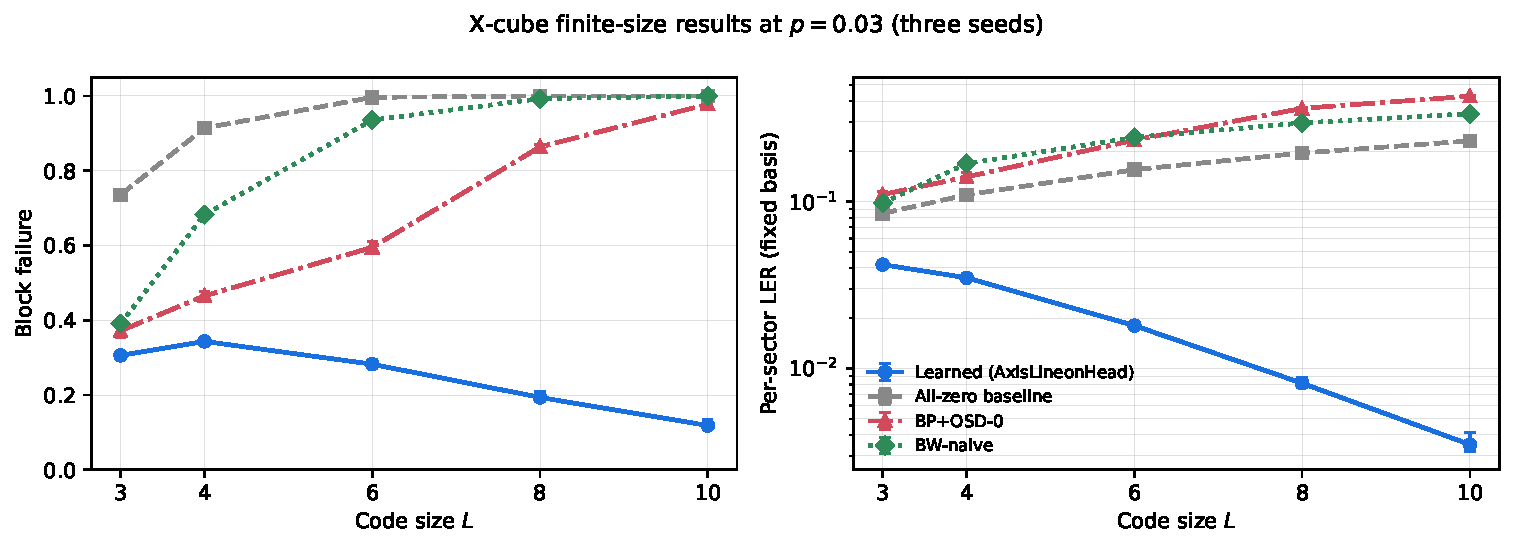
\includegraphics[width=\linewidth]{fig_scaling.pdf}
\caption{Finite-size performance at $p=0.03$ (3-seed means and
seed-bootstrap $95\%$ intervals; Table~\ref{tab:main}). Left: block failure,
which improves for the learned decoder from $L=4$ onward. Right: mean
per-sector error in the fixed logical basis, which improves at every
tested size. Each size has a separately trained model. Both panels use
the retained result JSONs without new experiments.}

\label{fig:scaling}
\end{figure}

\paragraph{Noise dependence and the unresolved crossing.}
Figure~\ref{fig:threshold} plots the measured dependence on $p$. For
$L\ge4$, larger sizes have lower block failure at $p=0.03$ and higher
block failure at $p=0.05$. This reversal motivates a denser noise sweep.
Except at $L=4$, however, only those two physical error rates were
measured. Lines between them are visual guides and do not establish a
threshold location or an asymptotic finite-size scaling law. A comparison
with the published Brown--Williamson or optimal-decoder thresholds
requires a resolved sweep, matched error sectors, and compatible failure
criteria~\cite{brown2019,song2021}. The $L=4$ high-noise sweep measures a
single size's advantage over a baseline; its disappearance cannot locate
a code threshold.

\begin{figure}[t]
\centering
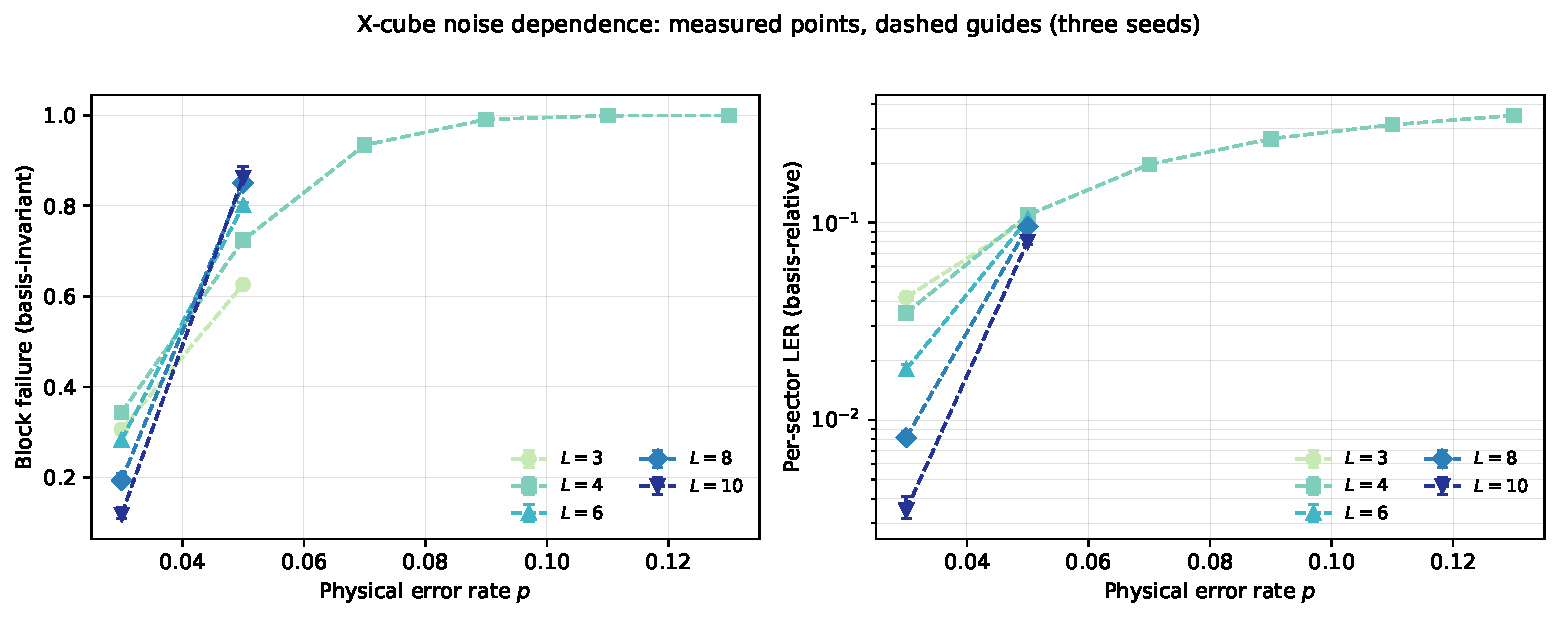
\includegraphics[width=\linewidth]{fig_threshold.pdf}
\caption{Measured learned-decoder error versus physical error rate
(3-seed means and seed-bootstrap $95\%$ intervals). Left: block failure.
Right: mean per-sector error in the fixed logical basis. Points are
measurements; dashed connectors are guides only. Except for $L=4$, each
curve has just two points, $p=0.03$ and $p=0.05$. No threshold is estimated
from their interpolation.}

\label{fig:threshold}
\end{figure}

\paragraph{Ablations and limits of the mechanism evidence.}
At $L=3$, $p=0.03$, seed 42, the global-pooling head has the same measured
block failure as the all-zero baseline ($0.7342$), whereas the coordinate
convolution and line-aggregation heads achieve $0.3022$ and $0.3026$
(Table~\ref{tab:ablation}). These measurements support preserving spatial
information in the readout. They do not show a unique advantage from line
aggregation, nor separate all differences in capacity and optimization.
Matched-capacity, multi-seed ablations at larger sizes are needed to test
whether explicit line aggregation offers an additional benefit.

The held-out radius-1 lookup has per-sector advantage over trivial of
$34.2\%$ at $L=3,p=0.03$, falling to $5.7\%$ at $L=4,p=0.03$, $0.1\%$
at $L=4,p=0.05$, and $\le0.3\%$ for all $L=6$ cells. The network
outperforms this finite-data control. Since the lookup is neither a
Bayes-optimal estimator nor an exhaustive family of local decoders, this
does not prove that all useful information lies outside its window.
The geometric mechanism remains a hypothesis supported by the architecture
and these restricted comparisons.

\begin{table}[t]
\centering
\small
\caption{Head ablation at $L=3$, $p=0.03$ (seed 42). Global pooling ties
trivial; structure-preserving heads win.}
\label{tab:ablation}
\begin{tabular}{lcc}
\toprule
Head & Block failure & Per-sector LER \\
\midrule
Trivial (floor)        & 0.7342 & 0.0846 \\
Global average pool    & 0.7342 & 0.0847 \\
Coordinate conv        & 0.3022 & 0.0420 \\
\textsc{AxisLineonHead}& 0.3026 & 0.0421 \\
\bottomrule
\end{tabular}
\end{table}

\paragraph{Predeclared win condition.} The fixed-in-advance criterion
(learned block-failure CI upper bound $0.6282$ below trivial CI lower bound
$0.8859$ at $L=3$, $p=0.05$) is satisfied.

\section{Related work}
\label{sec:related}
Neural decoders have been developed extensively for the surface and toric
codes, including equivariant architectures (The END~\cite{end2023}; the 3D-toric
equivariant ML decoder~\cite{toric3dequiv2024}, which shows weight-sharing is
necessary but not sufficient) and scalable CNNs for 3D/4D toric
codes~\cite{breuckmann2017}. For fracton codes specifically, prior decoding work
is \emph{algorithmic}: Brown--Williamson give a parallelized matching$+$BP
fracton decoder~\cite{brown2019} (threshold $\approx 4.3\%$), and the optimal
X-cube fracton-sector threshold under $X$-noise is
$\approx 7.5\%$~\cite{song2021}. Neural-network quantum states have been applied
to fracton \emph{ground states}~\cite{fracton-nqs2024} but not to decoding.
Our contribution is an X-cube-specific neural decoder and its released
finite-size benchmarks; we do not rely on a claim of priority. We benchmark it against the BW-naive implementation
of Brown--Williamson's code-specific matching framework~\cite{brown2019} described
in \S\ref{sec:methods}, alongside the trivial floor and BP+OSD-0. We distinguish it from the parallel line of work that
decodes high-rate qLDPC codes by \emph{algebraic} means: Wills et
al.~\cite{wills2026concat} concatenate a quantum Reed--Solomon outer code over a
bivariate-bicycle qLDPC inner code, decoded by list decoding and (Relay-)BP, with
no learned component --- a different code family \emph{and} a non-neural method.
Learned message-passing decoders for qLDPC and bivariate-bicycle codes also exist:
Astra~\cite{astra2024} uses a graph-neural/message-passing architecture on Tanner
graphs and reports extrapolation across code distances; it is complementary to
our X-cube-specific line-aggregation head rather than a prior fracton decoder.
Comprehensive surveys of the decoder landscape~\cite{spencer2026tutorial} confirm
that machine-learning decoders and fracton-adjacent topics are each individually
mainstream; our study focuses on their intersection in a particular code and noise model. The
self-correcting-memory motivation follows the fracton literature (Haah's
code~\cite{haah2011} and the partial-self-correction line).

\section{Discussion and limitations}
\label{sec:discussion}
The retained measurements demonstrate a learned decoder with improving
finite-size block recovery from $L=4$ through $L=10$ at $p=0.03$, together
with monotone improvement in the fixed-basis per-sector metric from $L=3$.
They also show the limit of that observation: block failure worsens with
size at $p=0.05$. All experiments use perfect syndrome measurements and
independent $X$ noise; noisy repeated measurements and other noise channels
are outside the present scope.

\paragraph{Objective and resource budget.}
Binary cross-entropy and validation selection optimize per-sector
prediction, not the joint logical-class decision. Joint or structured
logical prediction is a useful follow-up for block recovery. Weight
sharing keeps the network parameter count independent of $L$, but models
are trained separately at each $(L,p)$, and processing a larger lattice
requires more computation. We do not measure training-time or sample
complexity scaling and do not demonstrate zero-shot transfer.

\paragraph{Baselines and statistics.}
BP+OSD-0 is one general-purpose configuration; higher-order OSD and other
tuned variants are not benchmarked. BW-naive is a simplified implementation
whose logical performance has not been validated against the published
algorithm. Its poor large-size behavior must be audited before using it
to support claims about code-specific matching. Large paired test-set
differences establish gaps between the implemented decoders on the sampled
distribution, not between all methods in those families. Three training
seeds provide limited information about training variability; the reported
seed-bootstrap intervals should be read alongside individual-seed results
and test-shot counts rather than as precise population coverage estimates.

\paragraph{Next experiments.}
A dense common $p$ grid across sizes would test the apparent reversal in
block-failure ordering. A validated code-specific baseline and larger-size,
matched-capacity head ablations would strengthen the performance and
mechanism claims. The $L=4$ sweep already shows the per-sector advantage
over trivial narrowing from $0.110$ versus $0.172$ at $p=0.05$ to $0.267$
versus $0.274$ at $p=0.09$, and disappearing around $p=0.11$--$0.13$;
these are single-size comparisons, not threshold estimates.
Transfer to 3D toric or other quantum codes would test the broader
architectural idea, but the appropriate readout and baseline depend on
each code's logical operators and syndrome geometry.

The classical motivation remains useful: a prior and a compact constraint
description can support inference without specifying a unique microscopic
answer. Here the acceptable ambiguity is precisely stabilizer equivalence.
Recovering the correct logical class is the benchmark; constructing a
passive or self-correcting memory would require additional physical results.

\section*{Reproducibility}
{\sloppy
All numbers are emitted by reproducible scripts. The main grid, ablation, and
signal-existence oracle come from \texttt{reproduce\_xcube\_results.py} (output
\texttt{data/xcube\_L346\_gen.json}, with the $L\ge 8$ scaling rows in
\texttt{data/xcube\_L810\_gen.json}); the high-$p$ sweep from the same script
(\texttt{data/xcube\_L4\_psweep.json}); and the BW-naive baseline from the
consolidated $L\le 6$ run plus the parallel $L\ge 8$ CPU run
(\texttt{reproduce\_xcube\_bw\_hpc.py}), with the standalone
\texttt{data/xcube\_bw\_baseline.json} retained for provenance. Full
provenance, including the per-cell statistics of App.~\ref{app:stats}, is in
\texttt{REPRODUCIBILITY.md}. In the family release, these artifacts are grouped
with the X-cube and gauge-theorem code under the fracton module of the companion
repository.\par}

\appendix
\section{Per-cell confidence intervals and McNemar counts}
\label{app:stats}
Table~\ref{tab:stats} reports the seed-bootstrap $95\%$ confidence intervals on
block failure for the learned and BW-naive decoders, and the paired-McNemar
discordant counts $(b,c)$ on identical test shots ($b$ = shots the learned
decoder gets right while the comparison decoder gets them wrong; $c$ = the
reverse). All paired McNemar tests are overwhelmingly significant; the
continuity-corrected $\chi^2$ statistic (or an exact binomial test) gives
$p < 10^{-12}$ in every tabulated paired comparison (learned-vs-BW-naive is
tabulated for $L\le 6$ only; at $L\ge 8$ BW-naive is compared by aggregate
failure rate, not paired shot-by-shot). BP+OSD-0 is evaluated on the smaller
cost-limited subsets noted in Table~\ref{tab:main} ($2{,}000$ shots/seed through
$L=8$, $300$ at $L=10$); even at the smallest subset its block-failure Wilson
$95\%$ interval stays far from the learned value (e.g.\ at $L=10,p=0.03$,
BP+OSD-0 $0.978$, Wilson $[0.966,0.986]$ on $900$ shots, vs.\ learned $0.118$),
so the reported gaps vastly exceed the baseline sampling error.

\begin{table}[h]
\centering
\footnotesize
\caption{Per-cell block-failure $95\%$ CIs and paired-McNemar discordant counts
$(b,c)$ for the learned decoder against trivial, BP+OSD-0, and BW-naive (the last
for $L\le 6$; --- at $L\ge 8$, where BW-naive fails near-totally and is compared
by aggregate failure rate). $L\ge 8$ from task-parallel per-cell runs.}
\label{tab:stats}
\begin{tabular}{ll cc c ccc}
\toprule
 & & Learned bf & BW-naive bf & & \multicolumn{3}{c}{McNemar $(b,c)$} \\
\cmidrule(lr){3-4}\cmidrule(lr){6-8}
$L$ & $p$ & [95\% CI] & [95\% CI] & & vs.\ trivial & vs.\ BP+OSD-0 & vs.\ BW-naive \\
\midrule
3 & 0.03 & 0.306 [0.303, 0.308] & 0.391 [0.387, 0.394] & & (53294, 1794) & (511, 99) & (12648, 2499) \\
3 & 0.05 & 0.626 [0.624, 0.628] & 0.703 [0.699, 0.705] & & (33405, 2079) & (499, 115) & (12663, 3470) \\
4 & 0.03 & 0.343 [0.343, 0.344] & 0.682 [0.681, 0.685] & & (69620, 1154) & (988, 257) & (43529, 2852) \\
4 & 0.05 & 0.724 [0.720, 0.728] & 0.937 [0.936, 0.938] & & (31555, 719) & (859, 146) & (26963, 1399) \\
6 & 0.03 & 0.282 [0.272, 0.296] & 0.935 [0.934, 0.936] & & (85691, 31) & (2067, 218) & (78726, 369) \\
6 & 0.05 & 0.800 [0.796, 0.807] & 0.999 [0.999, 0.999] & & (23950, 11) & (1108, 22) & (23854, 30) \\
8 & 0.03 & 0.194 [0.183, 0.210] & 0.993 [0.992, 0.993] & & (72574, 0) & (4067, 23) & --- \\
8 & 0.05 & 0.850 [0.842, 0.856] & 1.000 [1.000, 1.000] & & (13485, 0) & (905, 0) & --- \\
10 & 0.03 & 0.118 [0.108, 0.134] & 1.000 [0.999, 1.000] & & (79351, 0) & (792, 1) & --- \\
10 & 0.05 & 0.863 [0.851, 0.887] & 1.000 [1.000, 1.000] & & (12337, 0) & (117, 0) & --- \\
\bottomrule
\end{tabular}
\end{table}

\begin{thebibliography}{99}

\bibitem{vijay2016} S. Vijay, J. Haah, and L. Fu.
\newblock Fracton topological order, generalized lattice gauge theory, and duality.
\newblock {\em Phys.~Rev.~B}, 94:235157, 2016. arXiv:1603.04442.

\bibitem{haah2011} J. Haah.
\newblock Local stabilizer codes in three dimensions without string logical operators.
\newblock {\em Phys.~Rev.~A}, 83:042330, 2011. arXiv:1101.1962.

\bibitem{pretko2017} M. Pretko.
\newblock Subdimensional particle structure of higher rank $U(1)$ spin liquids.
\newblock {\em Phys.~Rev.~B}, 95:115139, 2017. arXiv:1604.05329.

\bibitem{song2021} H. Song et al.
\newblock Optimal thresholds for fracton codes and random spin models with subsystem symmetry.
\newblock arXiv:2112.05122, 2021. (Optimal X-cube fracton-sector threshold $\approx 7.5\%$.)

\bibitem{brown2019} B.~J. Brown and D.~J. Williamson.
\newblock Parallelized quantum error correction with fracton topological codes.
\newblock {\em Phys.~Rev.~Research}, 2:013303, 2020. arXiv:1901.08061.

\bibitem{end2023} E.~Egorov, R.~Bondesan, and M.~Welling.
\newblock The END: An equivariant neural decoder for quantum error correction.
\newblock arXiv:2304.07362, 2023.

\bibitem{toric3dequiv2024} O.~Weissl and E.~Egorov.
\newblock Equivariant machine learning decoder for 3D toric codes.
\newblock arXiv:2409.04300, 2024. (Weight-sharing necessary but not sufficient.)

\bibitem{breuckmann2017} N.~P. Breuckmann and X. Ni.
\newblock Scalable neural network decoders for higher dimensional quantum codes.
\newblock {\em Quantum}, 2:68, 2018. arXiv:1710.09489.

\bibitem{fracton-nqs2024} M.~Machaczek, L.~Pollet, and K.~Liu.
\newblock Neural quantum state study of fracton models.
\newblock arXiv:2406.11677, 2024. (Ground states, not decoding.)

\bibitem{astra2024} A.~S. Maan and A.~Paler.
\newblock Machine learning message-passing for the scalable decoding of QLDPC codes.
\newblock arXiv:2408.07038, 2024.

\bibitem{wills2026concat} A.~Wills, M.~E. Beverland, L.~S. Bishop, J.~M. Gambetta, P.~Rall, V.~Siddhu, and A.~W. Cross.
\newblock Concatenating algebraic codes over high-rate quantum {LDPC} codes.
\newblock arXiv:2605.21898, 2026.

\bibitem{spencer2026tutorial} D.~J. Spencer, S.~P. Jain, A.~Tanggara, Z.~Sun, T.~Haug, D.~Khu, and K.~Bharti.
\newblock Quantum error correction and fault tolerance: A comprehensive tutorial.
\newblock arXiv:2605.29137, 2026.

\end{thebibliography}

\end{document}

